\documentclass[11pt]{iopart}
%Uncomment next line if AMS fonts required
%\usepackage{iopams}
\usepackage{fancyhdr}
\usepackage{graphicx}
\usepackage{todonotes}
\usepackage{subfig}
\usepackage{ulem}
\usepackage{amssymb}
\usepackage{multicol}

\usepackage[hidelinks]{hyperref}
\hypersetup{colorlinks=false}

\pagestyle{fancy}
\lhead{Diffusion Limited Aggregation}
\rhead{Candidate Number: 21594}

\begin{document}

%Makes TODO notes format properly in margin
\setlength{\marginparwidth}{1.5cm}

\title[]{Thermodynamics and Diffusion Limited Aggregation}

\author{Candidate Number: 21594}

\address{Department of Physics,
University of Bath, Bath BA2 7AY, United Kingdom}
\begin{abstract}
Abstract goes here
\end{abstract}

%\listoftodos

%Uncomment for PACS numbers title message
%\pacs{00.00, 20.00, 42.10}
% Keywords required only for MST, PB, PMB, PM, JOA, JOB? 
%\vspace{2pc}
%\noindent{\it Keywords}: Article preparation, IOP journals
% Uncomment for Submitted to journal title message
%\submitto{\JPA}
% Comment out if separate title page not required
%\maketitle

\section*{Preface}
Although the coursework was initially presented as a C++ project, I took the liberty of rewriting the DLA system in a programming language called Google Go. The motivation for this is Go more easily supports high concurrency. This means that instead of simulating 1 cluster at a time, 100 different clusters can be simulated simultaneously in different threads. To support this high level of concurrency, the results were generated by running the code on a 32-core virtual server. The code is accessible on Github: https://goo.gl/fDia6z.

\section{Introduction and Simulation Method}

Diffusion Limited Aggregation (DLA) is a theory that models the process of how clusters of particles form in systems where growth is driven primarily by diffusion \cite{dla}. DLA theory is applicable to systems including Hele-Shaw flow \cite{heleshaw}, electrodeposition \cite{electrodeposition} and dielectric breakdown \cite{electricbreakdown}.

\begin{figure}[b]
  \centering
  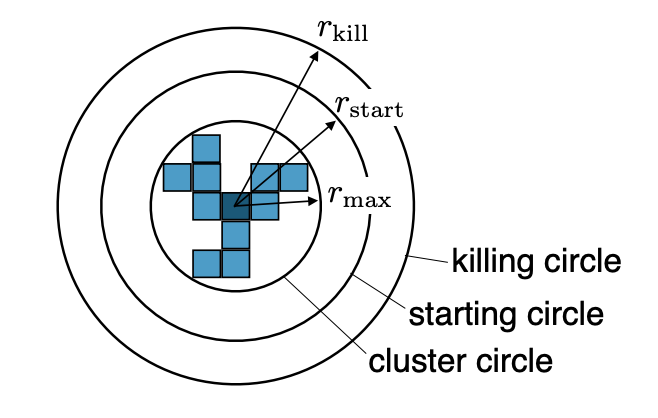
\includegraphics[width=0.5\linewidth]{images/circles.png}
  \caption{"Diagram of the circles used in the DLA code. The initial particle is shown in dark blue, and all circles are centred on this particle. There are three circles which indicate the approximate cluster size ('cluster circle'), the locations at which particles are introduced to the system ('starting circle'), and the points at which particles are removed from the system, to prevent them from wandering too far from the cluster ('killing circle')." Diagram and caption lifted verbatim from \cite{handout}.}
  \label{fig:circles}
\end{figure}

In the DLA method used in this paper, a stationary seed particle is placed at the centre of a regular square lattice. This seed particle defines the origin of our system, as shown in Figure 1. A particle is then added to the system at a radius $r_{start}$ from the origin. This radius is computed such that each new particle is added at a radius greater than the radius of any stationary particle in the system. Diffusion limited transport is driven by Brownian motion \cite{brownian}, a random process, so the new particle is made to undergo a Markovian random walk through the system. If the particle moves to a cell on the lattice that is horizontally or vertically adjacent to a stationary particle, the particle is stuck to the grid cell with a sticking probability $p_{stick}$. If the particle moves too far away from the cluster, as defined by a radius $r_{kill}$, the particle is removed from the system. This is done to increase the time efficiency of the program, as it removes the possibility of a particle moving into regions of space where the probability of sticking to the cluster in any reasonable number of further steps is extremely small. Once a particle is stuck to the cluster or killed for 'walking' too far away, a new particle is added on the start circle and the process is repeated. The simulation is terminated when the border of the cluster approaches the edge of the fixed-dimension grid or when the total number of particles in the cluster reaches a predefined limit.

In this paper, it is tested to see if the maximum number of particles used in a DLA system affects the fractal index of the generated cluster. Enquiry is also made into how fractal dimension depends on the sticking probability $p_{stick}$, as this links to the thermodynamics of physical systems that can be modelled using DLA.

\section{Method}
\subsection{Random Walks and Ensemble Averaging}
To simulate the Brownian motion of diffusing particles, DLA simulations have free particles undergo a random walk. For each iteration, the direction a particle attempts to move in is parameterized by a discrete random variable $D \sim$ $\mathcal{U}\{0, 3\}$ $\cap$ $\mathbb{Z}$ , with each value of $D$ corresponding to one of the particle's degrees of freedom - 2 horizontal and 2 vertical. The issue with this is that the sequence of random numbers generated by the algorithm used in the DLA simulations is only 'pseudo-random'. For a given random number generator seed, the same sequence of numbers will always be generated, which may bias the results of the simulations. To mitigate this, an ensemble of systems are simulated independently, each with a different random number generator seed. For a given measurement $\xi(t)$, an ensemble average $\overline{\xi(t)}$ is calculated by averaging measurements from each of these $n$ systems $\{i\}_1^n$, where $i$ represents a specific simulated system:


\begin{equation}
\label{averageequation}
\overline{\xi(t)} = \frac{1}{n}\sum_{i=1}^{n}{\xi_i(t)}
\end{equation}
%Standard error $\sigma_{\overline{\xi}}$ can be used as a measure of how close the ensemble average is to the true value:

%\begin{equation}
%\sigma_{\overline{\xi}} = \frac{1}{\sqrt{n-1}} \left[ \overline{\xi(t)^2} - \overline{\xi(t)}^2 \right]^{1/2}
%\end{equation}

\subsection{Determining the Fractal Dimension of DLA Aggregates}

DLA clusters are fractal objects \cite{dla}. This means their geometric structure can be described by a measure called 'fractal index', $d_f$. For a given DLA system, the fractal dimension is implicitly defined by \cite{handout}

\begin{equation}
N_c(r_{max}) = (\alpha \cdot r_{max})^{d_f} + \beta
\end{equation} 
where $\alpha$, $\beta$ and $d_f$ are free parameters.
Taking logs of both sides and differentiating with respect to $\ln r_{max}$ yields the relationship

\begin{equation}
\frac{d(\ln r_{max})}{d(\ln N_c)} = \frac{1 + \beta/(\alpha \cdot r_{max})^{d_f}}{d_f}
\end{equation} 
which in the limit of large $r_{max}$ gives
\begin{equation}
\label{dflogequation}
\lim_{r_{max}\to\infty} \frac{d(\ln r_{max})}{d(\ln N_c)}  = \frac{1}{d_f}
\end{equation}
which can be used to trivially determine the fractal dimension of a simulated DLA system.

\subsection{Sticking Probabilities}

DLA systems can be setup so that the sticking probability $p_{stick}$ is less than 1, indicating that a particle may sometimes collide with a cluster and recoil. This may be useful when studying systems with a high thermodynamic temperature, where free particles on average have higher kinetic energies as described by a Maxwellian distribution, for example. To achieve this, when the system determines that a particle has moved into a grid cell where there is the possibility of 'sticking', a random number $p$ is sampled from a continuous uniform distribution $P \sim$ $\mathcal{U}\{0, 1\}$. If $p \leq p_{stick}$ then the particle is marked as stationary and the system proceeds to add a new particle. In the case $p > p_{stick}$, the particle remains in the grid cell adjacent to the cluster but is not marked as stationary. The system then proceeds to generate a new random direction to attempt to move the particle in. If the algorithm tries to move the free particle into a grid cell that is occupied by a cluster cell, the move is rejected and a new random direction is generated until a successful move is made.

\section{Results}

\subsection{Determining the Fractal Dimensions of DLA Aggregates}

\begin{figure}[t]
  \centering
  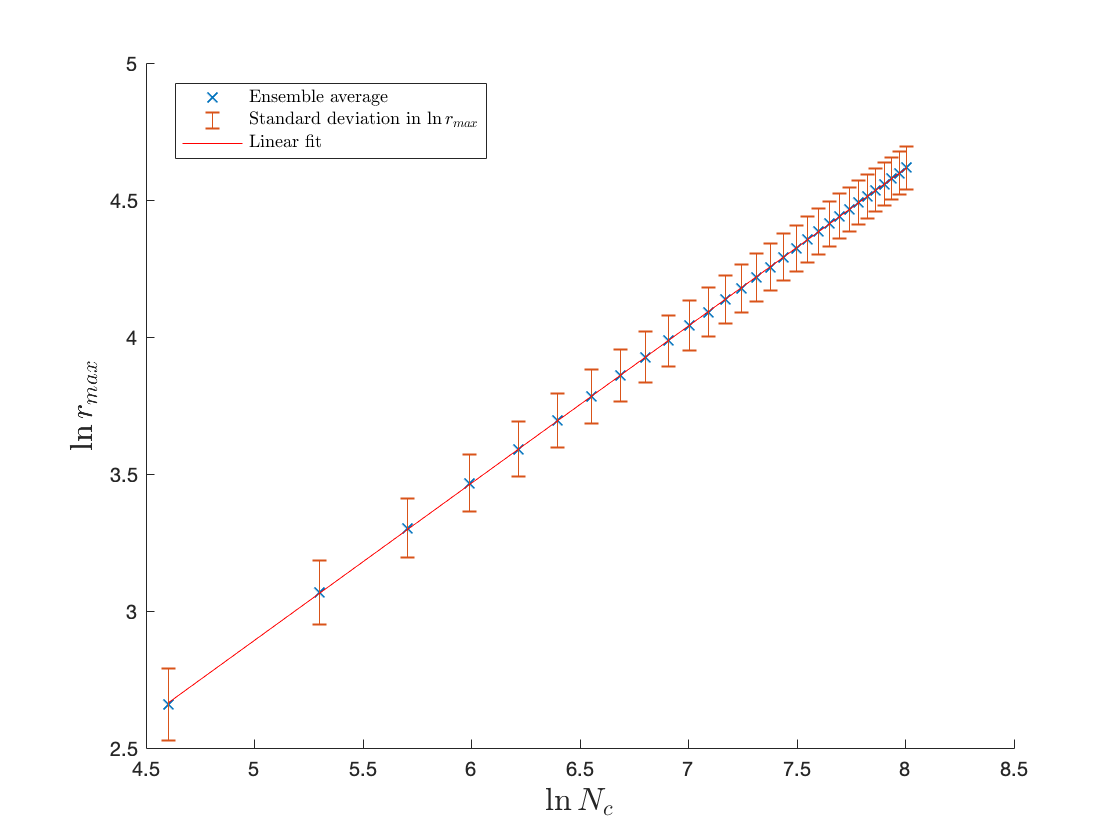
\includegraphics[width=0.8\linewidth]{images/loggraph.png}
  \caption{Natural log of cluster radius, $r_{max}$, as a function of the natural log of the number of particles in the cluster, $N_c$. Data points represent average over 1000 subsystems using equation \ref{averageequation}. Error bars represent the standard deviation in the values of $\ln r_{max}$. Application of equation \ref{dflogequation} yields $d_f = 1.743  \pm 0.003$.}
  \label{fig:loggraph}
\end{figure}

Figure \ref{fig:loggraph} shows the ensemble average of the natural log of the cluster radius as a function of the natural log of the number of particles in the DLA cluster, averaged over $n=1000$ independent systems with different random number generator seeds. Application of equation \ref{dflogequation} yields a fractal dimension for 2D DLA systems of $d_f = 1.743 \pm 0.003$.

\subsection{Self Similarity}

Figure \ref{fig:selfsimilar} shows graphical representations of the results of a DLA simulation with 3000 particles. Figure \ref{fig:selfsimilar} (a) shows the entire cluster and Figure \ref{fig:selfsimilar} (b) shows the bounded area from (a) magnified. Observe how all the major branching points in Figure \ref{fig:selfsimilar} (b) have exactly two child branches - one emerging downwards and one emerging to the left. This demonstrates the fractal and self-similar nature of the simulated DLA clusters.

\begin{figure}[t]
    \centering
    \subfloat[Simulated DLA Cluster]{{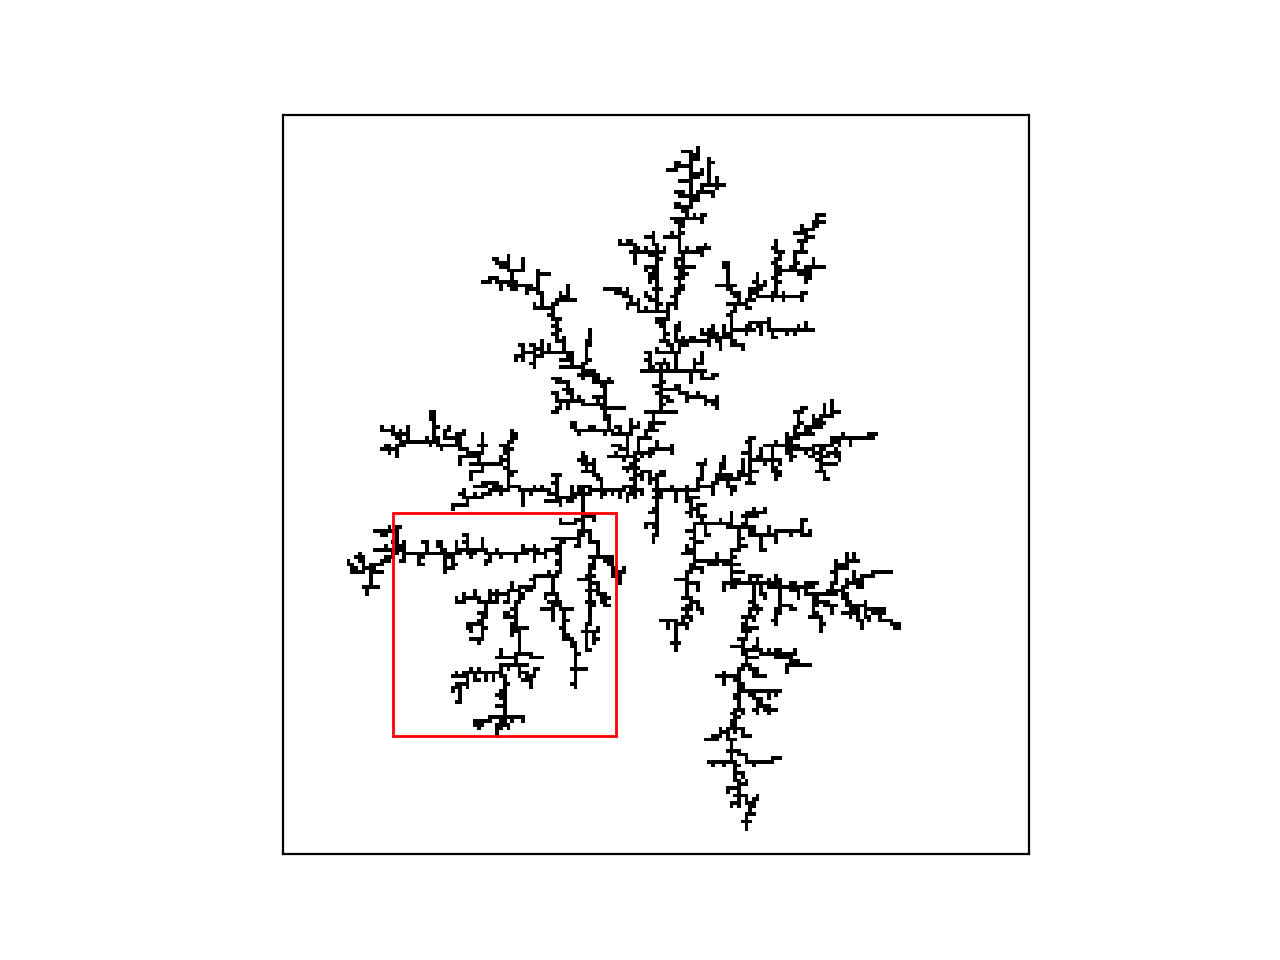
\includegraphics[width=8cm]{images/cluster.png} }}\quad
     \subfloat[Magnification of lower left branch]{{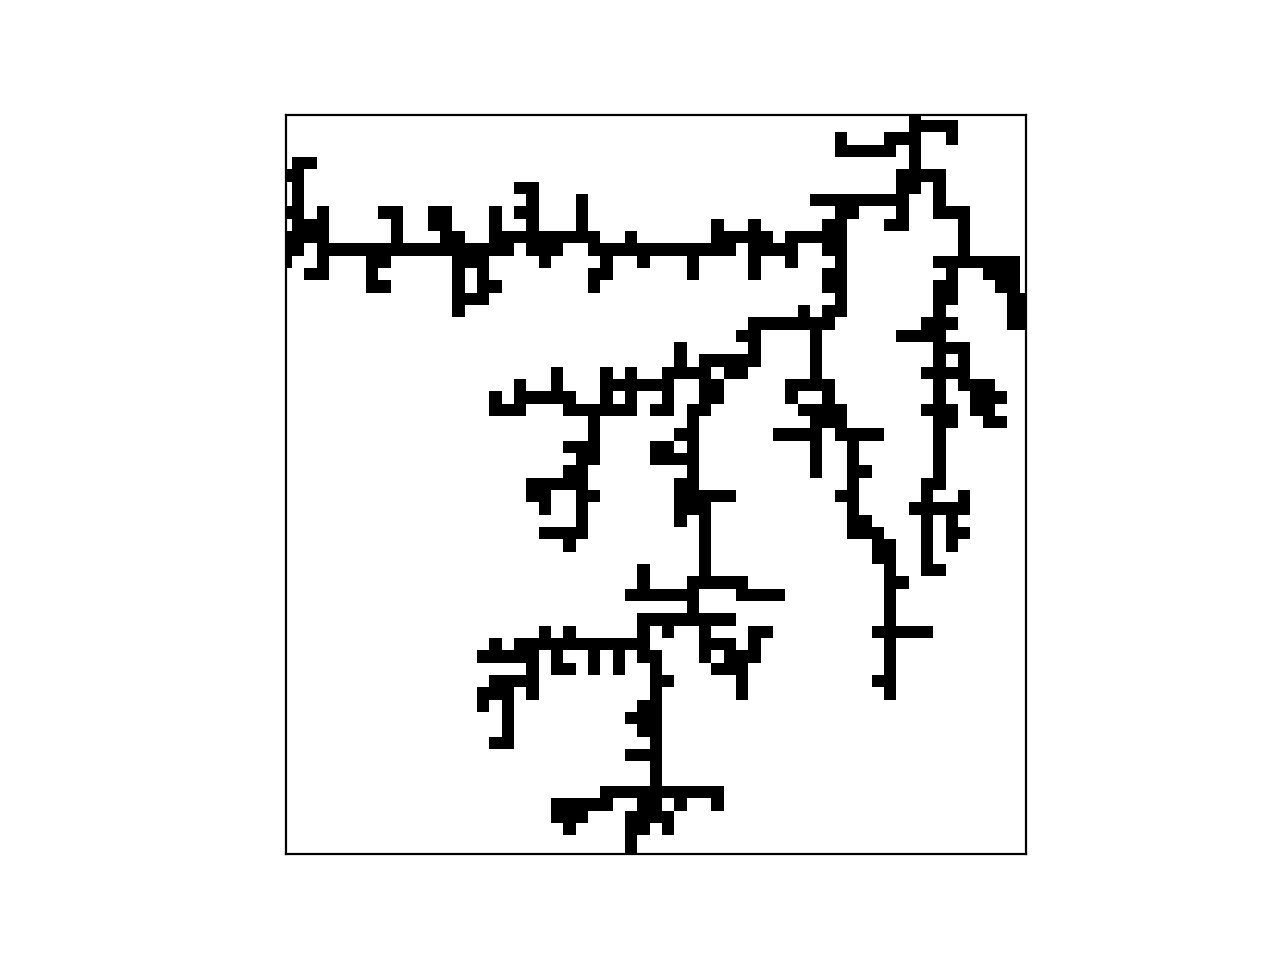
\includegraphics[width=8cm]{images/Zoomed.png} }}\\
 
    \caption{Graphical representation of a simulated DLA cluster with 3000 particles and a sticking probability of $p_{stick} = 1.0$. (a) shows the entire DLA cluster and (b) shows a magnification of the bordered section in (a).}
    \label{fig:selfsimilar}
\end{figure}

\subsection{Sticking Probabilities}

\section{Discussion}
\subsection{Determining the Fractal Dimension of DLA Aggregates}

The fractal dimension of the simulated 2D DLA clusters for sufficiently large cluster radius converges on $1.743 \pm 0.003$. This is in agreement with the literature value for 2D DLA clusters of 1.7\cite{fractalindexref}. This indicates that the simulation algorithm presented here sufficiently models the behaviour of physical DLA systems.

\subsection{Geometric Comparison with Experimental Results}

\begin{figure}[t]
    \centering
    \subfloat[Simulated DLA Cluster]{{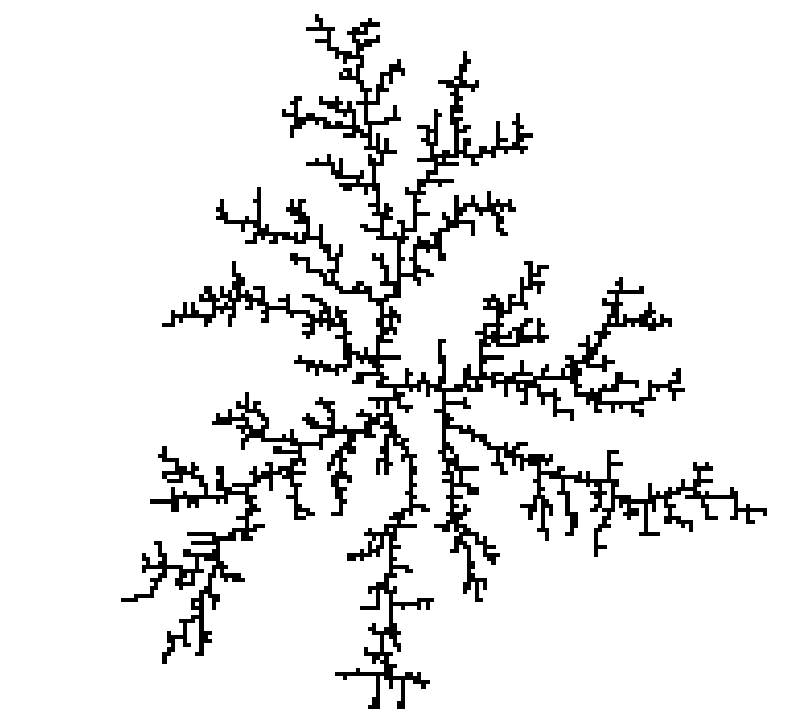
\includegraphics[width=6cm]{images/cluster2.png} }}\quad
     \subfloat["A zinc electrodeposit produced in a thin cell" \cite{dla}]{{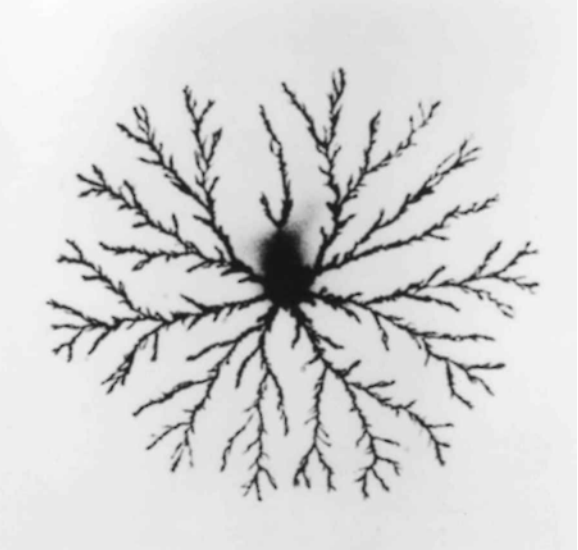
\includegraphics[width=5cm]{images/zinc.png} }}\\
 
    \caption{Comparison of a simulated DLA cluster (3000 particles, $p_{stick} = 1.0$) with an experimentally produced zinc electrodeposit as presented in \cite{dla}.}
    \label{fig:realcrystal}
\end{figure}

Figure \ref{fig:realcrystal} compares a simulated DLA cluster with an experimentally produced zinc electrodeposit - a system for which diffusion is the primary transport method, meaning DLA theory is applicable \cite{dla}. Both clusters demonstrate growth around a central attractor, with both clusters having visually similar radial branching patterns. The number of first order branches originating from the centre is greater in the experiment than in the simulated example, which could be explained by the greater surface area of the attractor in the experiment (the central electrode is not a point particle unlike the centre particle in the simulation), meaning more particles can become attached. Another consideration is that, experimentally, diffusing particles are free to attach to a cluster particle at any arbitrary angle $\theta \in \{\mathcal{R} \cap [0, 2\pi) \}$ (neglecting possible chemical lattice constrains), whereas in the simulation we enforce a square lattice, with free particles only attaching if they are directly horizontally or vertically adjacent to a cluster particle, thus enforcing the unnatural constraint $\theta = m\pi/2, m \in [0,3]$. This could be mitigated by allowing diagonal attachment and could be verified by further investigating the effect, if any, of simulating DLA clusters with different lattice arrangements. However, determining if lattice arrangement affects the geometry of the produced clusters would require a more sophisticated method of quantifying the distribution and arrangement of the cluster branches, which is outside the scope of this paper.  More simply, the case here could also be that, due to DLA simulations being stochastic, the same simulation setup with a different random number generator seed could produce a greater (or indeed fewer) number of branches -  with the number of branches simply being 'random'.

\subsection{Suggestions for Improvement}
Although seemingly effective, the implementation of the kill circle could be somewhat naive. If a particle walks outside of the kill circle it is, at present, simply terminated, and a new particle is added at random anywhere on the start circle. It may be more prudent to consider the probability of where the wandered particle is likely to reappear at a future instance of time as there could be a radial bias to the reappearance position, depending on the angle the particle wanders away from the system at. However, this is likely not significant as it could be expected that any radial bias would be averaged out over time because the probability distribution of the angle $\theta$ that the particle walks away from the system at is uniform.  Not withstanding this, a more sophisticated alternative using Green's functions and probability densities is presented in section 7.1 of "Diffusion-limited aggregation: A kinetic critical phenomenon?"\cite{dla2}. 
Another trivial but potentially significant improvement is the addition of adaptive step sizes.

\section{Conclusion}
bla

\section*{References}
\bibliography{refs}
\bibliographystyle{plain}

\end{document}

